\documentclass[10pt]{beamer}
\usetheme[progressbar=frametitle]{metropolis}
\usepackage{appendixnumberbeamer}
\usepackage{booktabs}
\usepackage[scale=2]{ccicons}
% \usepackage[ngerman]{babel}
\usepackage{graphicx} 
\graphicspath{{images/}{../images/}}
\usepackage{tikz} 
\usepackage{wrapfig}
%\usepackage[utf8]{inputenc}
%\usepackage[T1]{fontenc}
\usepackage{moreverb}
\usepackage[backend=biber]{biblatex}   
\addbibresource{content/cites.bib}
%\bibliography{content/cites.bib}
\usepackage{textcomp}
%\usepackage{fontspec}
%\setsansfont{Fira Sans}
\usepackage{hyperref}
\usepackage{animate}
\renewcommand*{\bibfont}{\scriptsize}
\usepackage[absolute,overlay]{textpos}

\setbeamercolor{framesource}{fg=gray}
\setbeamerfont{framesource}{size=\tiny}
%\usepackage{caption}
%\captionsetup[figure]{labelformat=empty}% redefines the caption setup of the figures environment in the beamer class.

\title{Final Presentation}
\author{András Czuczi, Samy Dafir, Andreas Lindlbauer} %#nohomo
\date{}
\usebackgroundtemplate

\newcommand{\source}[1]{\begin{textblock*}{4cm}(8.7cm,8.6cm)
    \begin{beamercolorbox}[ht=0.5cm,right]{framesource}
        \usebeamerfont{framesource}\usebeamercolor[fg]{framesource} Source: {#1}
    \end{beamercolorbox}
\end{textblock*}}
\begin{document}

\begin{frame}
	\maketitle 
\end{frame}

%%%%%%%%%%%%%%%%%%%%%%%%%%%%%%%%%%%%%%%%%%%%%%%%%%%%%%%%%%%%%%%%%%%%%%%%%%%%%%%%%%%%%%%%%%%%%%%%

\begin{frame}{Overview}
	\tableofcontents
\end{frame}

%%%%%%%%%%%%%%%%%%%%%%%%%%%%%%%%%%%%%%%%%%%%%%%%%%%%%%%%%%%%%%%%%%%%%%%%%%%%%%%%%%%%%%%%%%%%%%%%

\section{Short summary of theme}
{
    \usebackgroundtemplate{\includegraphics[width=\paperwidth,height=\paperheight]{ars.jpg}}
\begin{frame}{Short summary of theme}
%    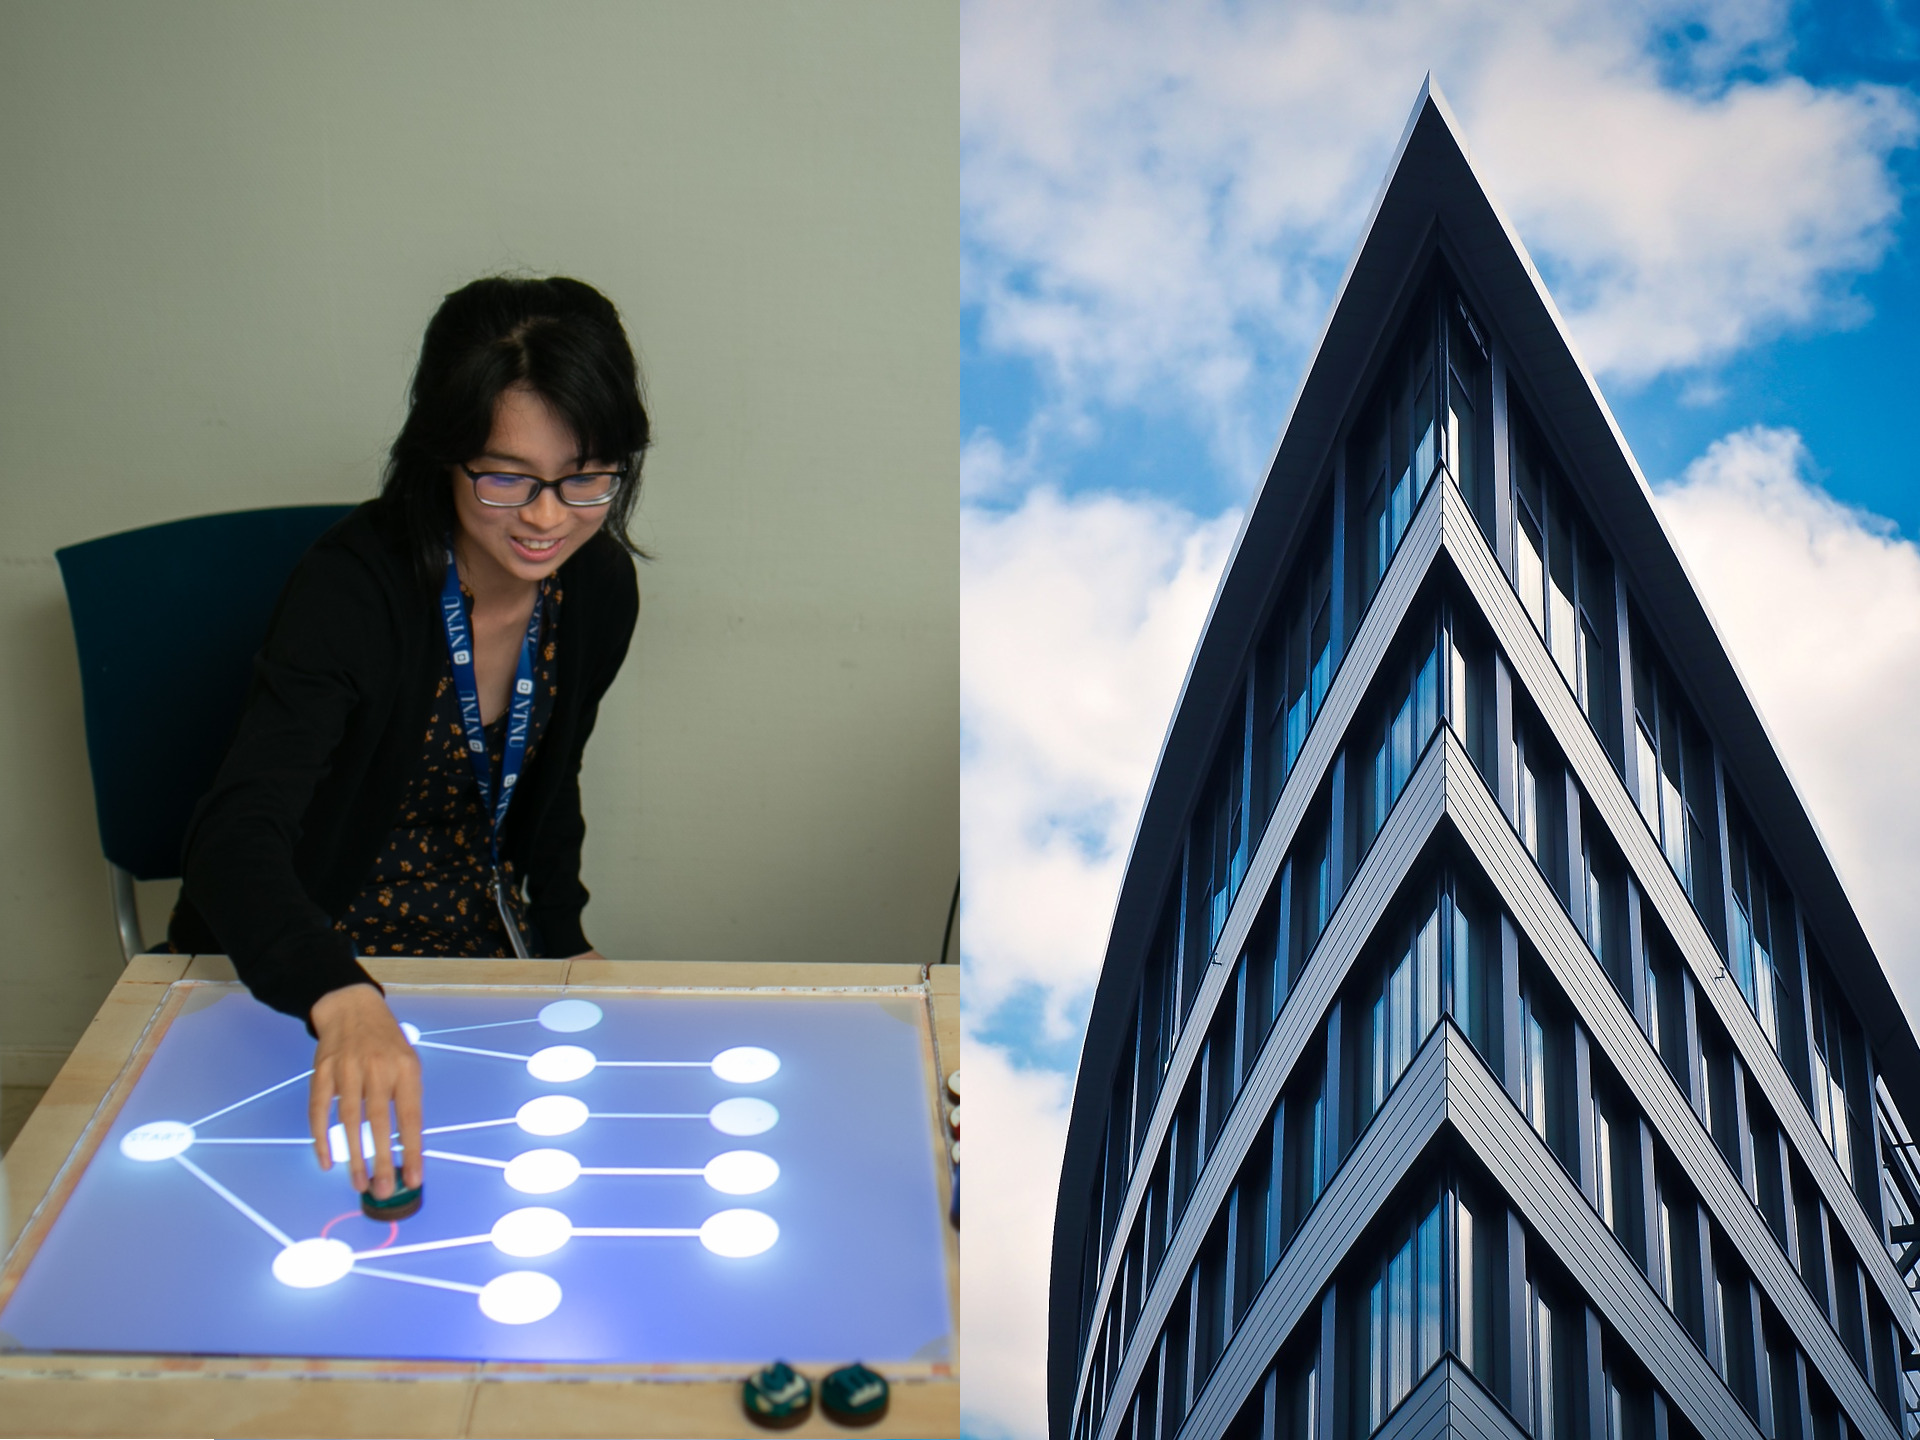
\includegraphics[width=\paperwidth,height=\paperheight]{interarch.jpg}%
%	\begin{block}{Intersection of architecture and interaction design}
\source{CC BY-SA 3.0 Walter Isack}
\end{frame}
}
%%%%%%%%%%%%%%%%%%%%%%%%%%%%%%%%%%%%%%%%%%%%%%%%%%%%%%%%%%%%%%%%%%%%%%%%%%%%%%%%%%%%%%%%%%%%%%%%



%%%%%%%%%%%%%%%%%%%%%%%%%%%%%%%%%%%%%%%%%%%%%%%%%%%%%%%%%%%%%%%%%%%%%%%%%%%%%%%%%%%%%%%%%%%%%%%%

\section{Short summary of literature review}

%%%%%%%%%%%%%%%%%%%%%%%%%%%%%%%%%%%%%%%%%%%%%%%%%%%%%%%%%%%%%%%%%%%%%%%%%%%%%%%%%%%%%%%%%%%%%%%%


{
    \usebackgroundtemplate{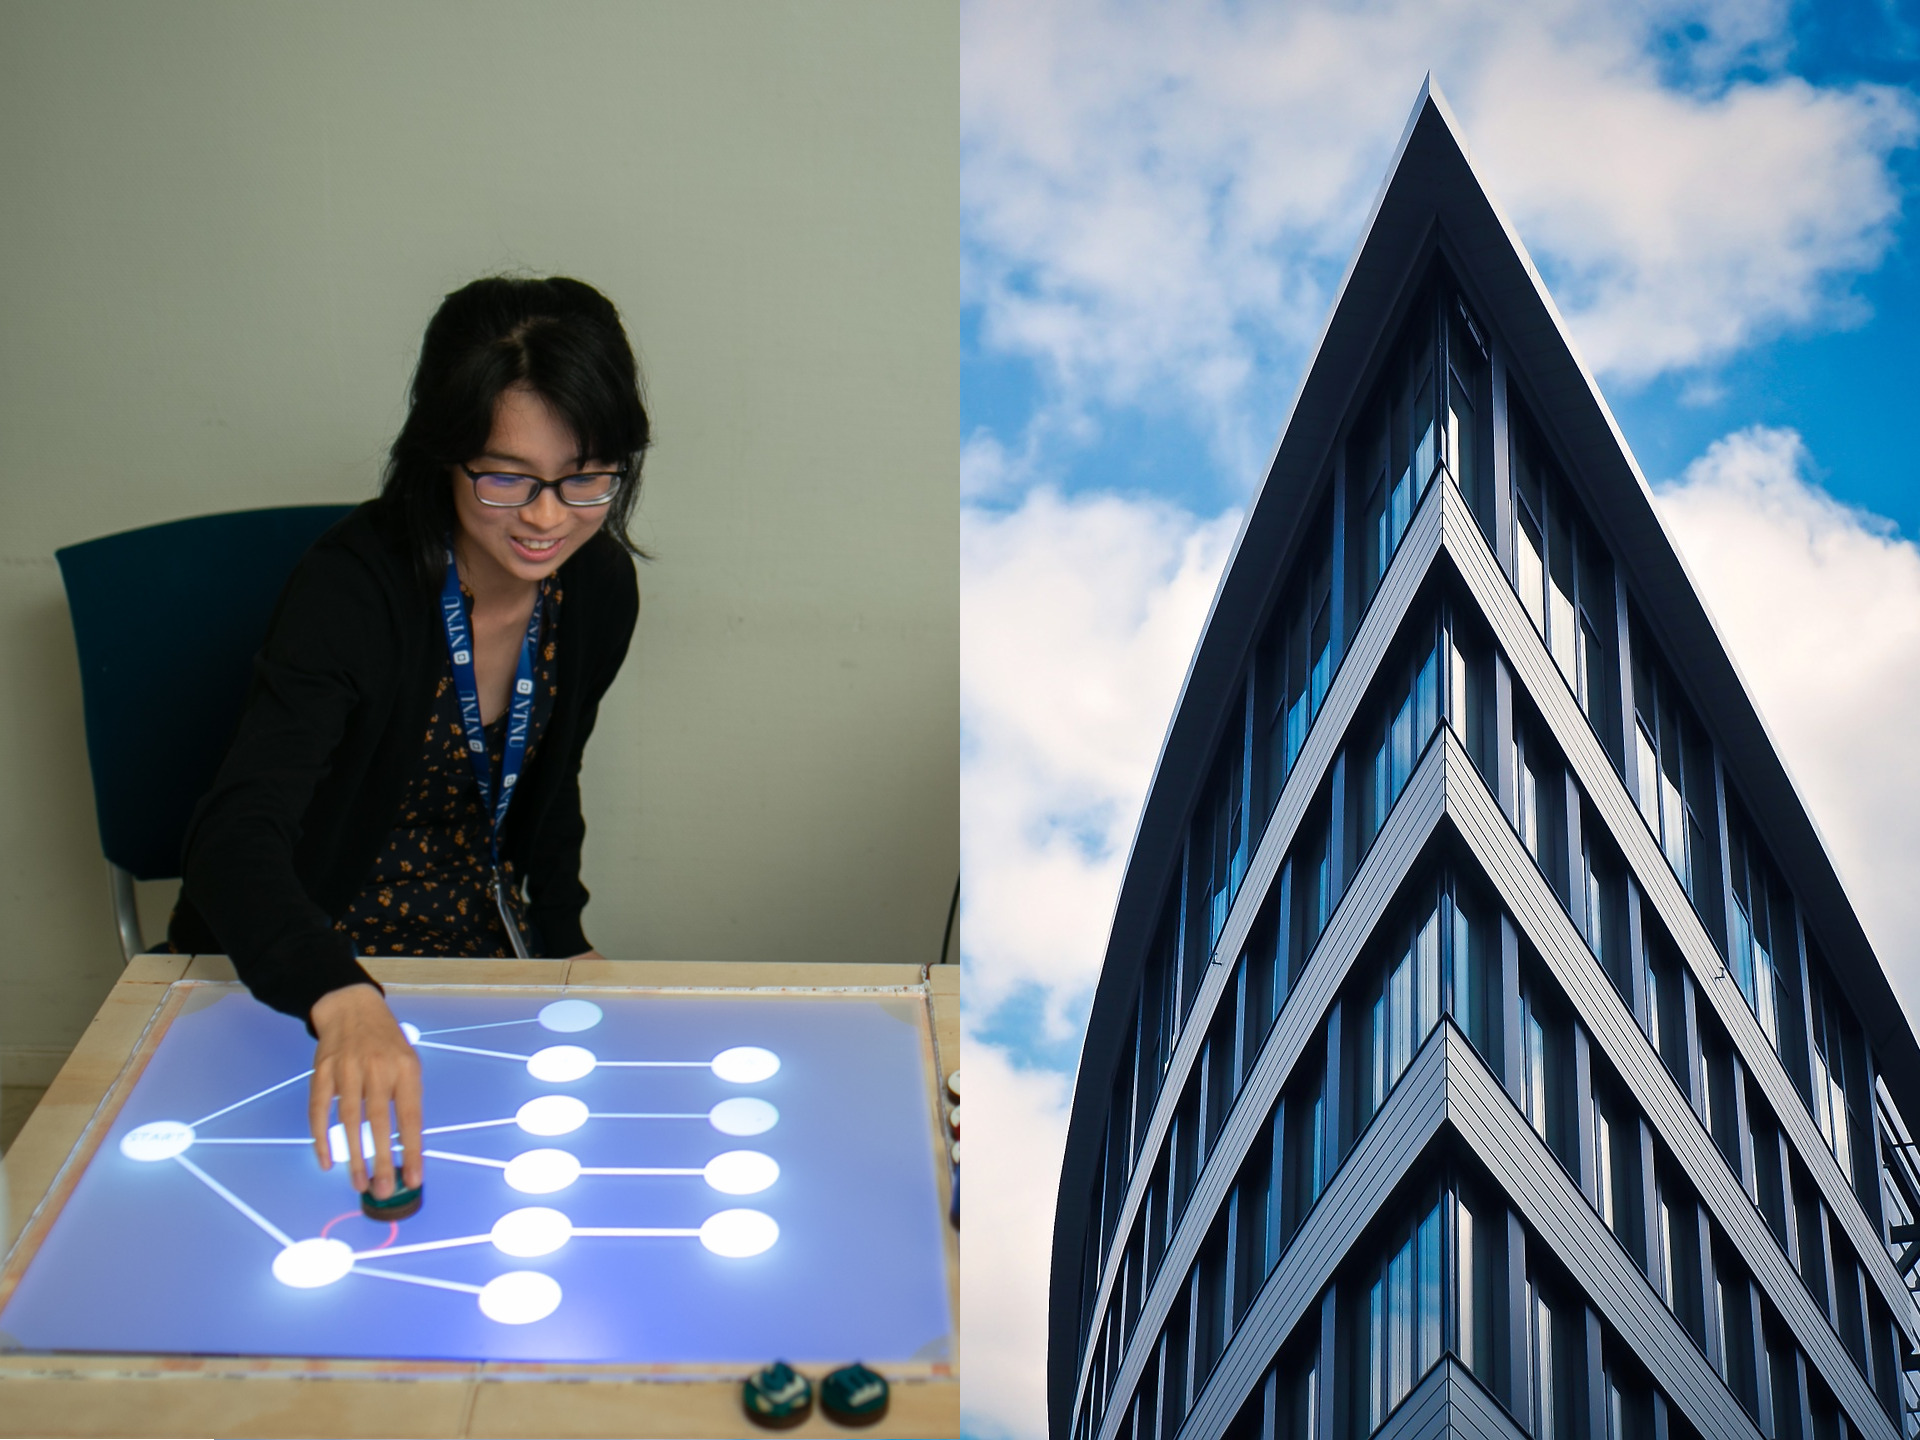
\includegraphics[width=\paperwidth]{interarch.jpg}}
\begin{frame}{Intersection of interaction design and architecture}
%    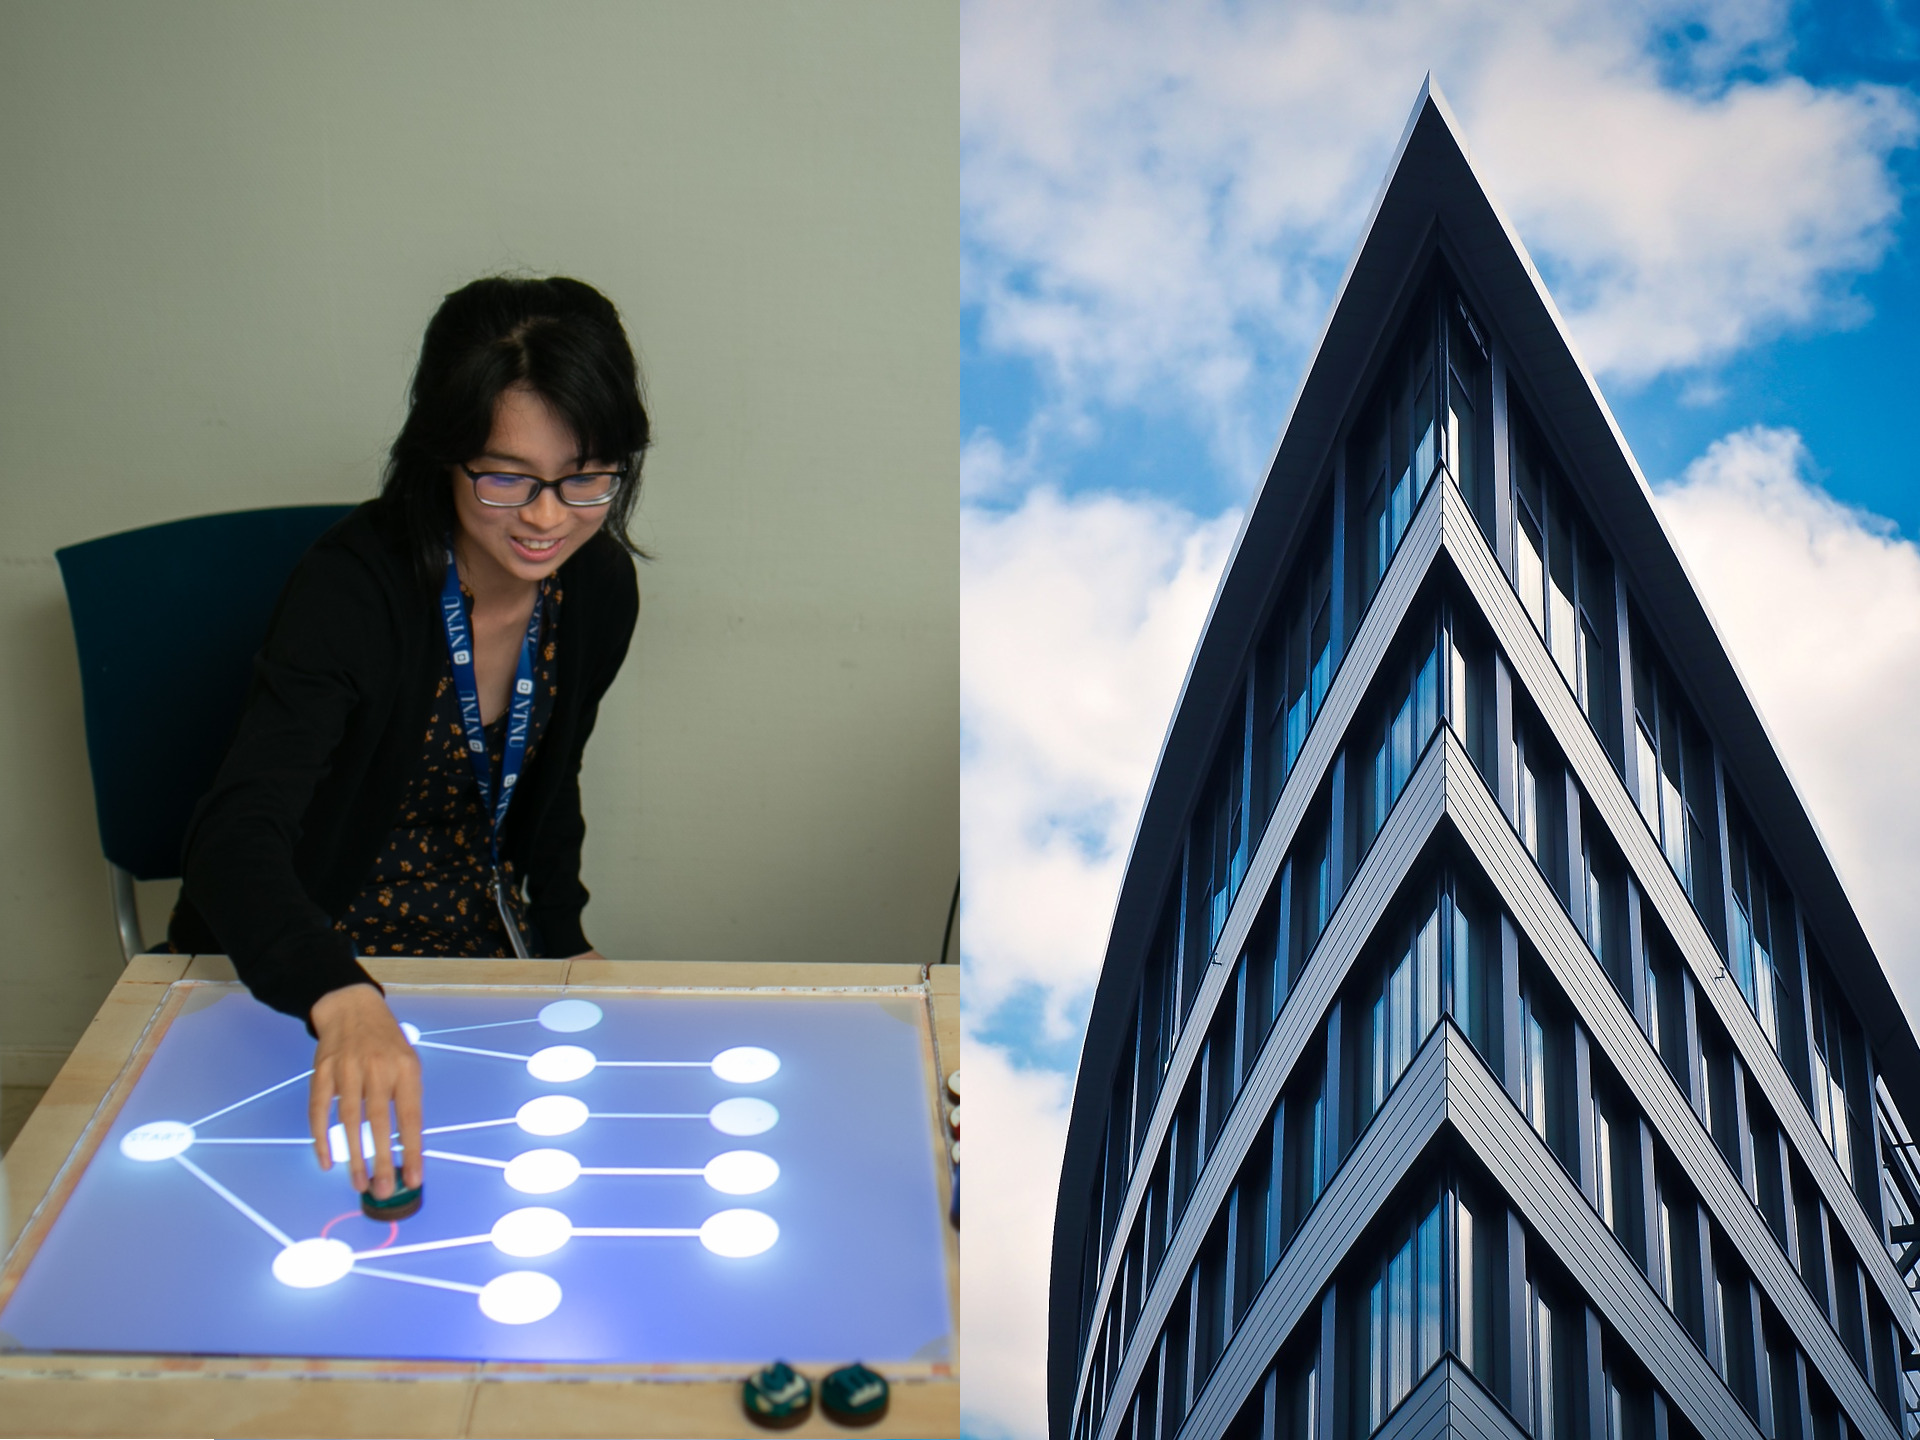
\includegraphics[width=\paperwidth,height=\paperheight]{interarch.jpg}%
%	\begin{block}{Intersection of architecture and interaction design}
\source{CC BY-NC 2.0 Kai T. Dragland \\ Pixabay License Michael Gaida}
\end{frame}
}

%%%%%%%%%%%%%%%%%%%%%%%%%%%%%%%%%%%%%%%%%%%%%%%%%%%%%%%%%%%%%%%%%%%%%%%%%%%%%%%%%%%%%%%%%%%%%%%%

{
    \usebackgroundtemplate{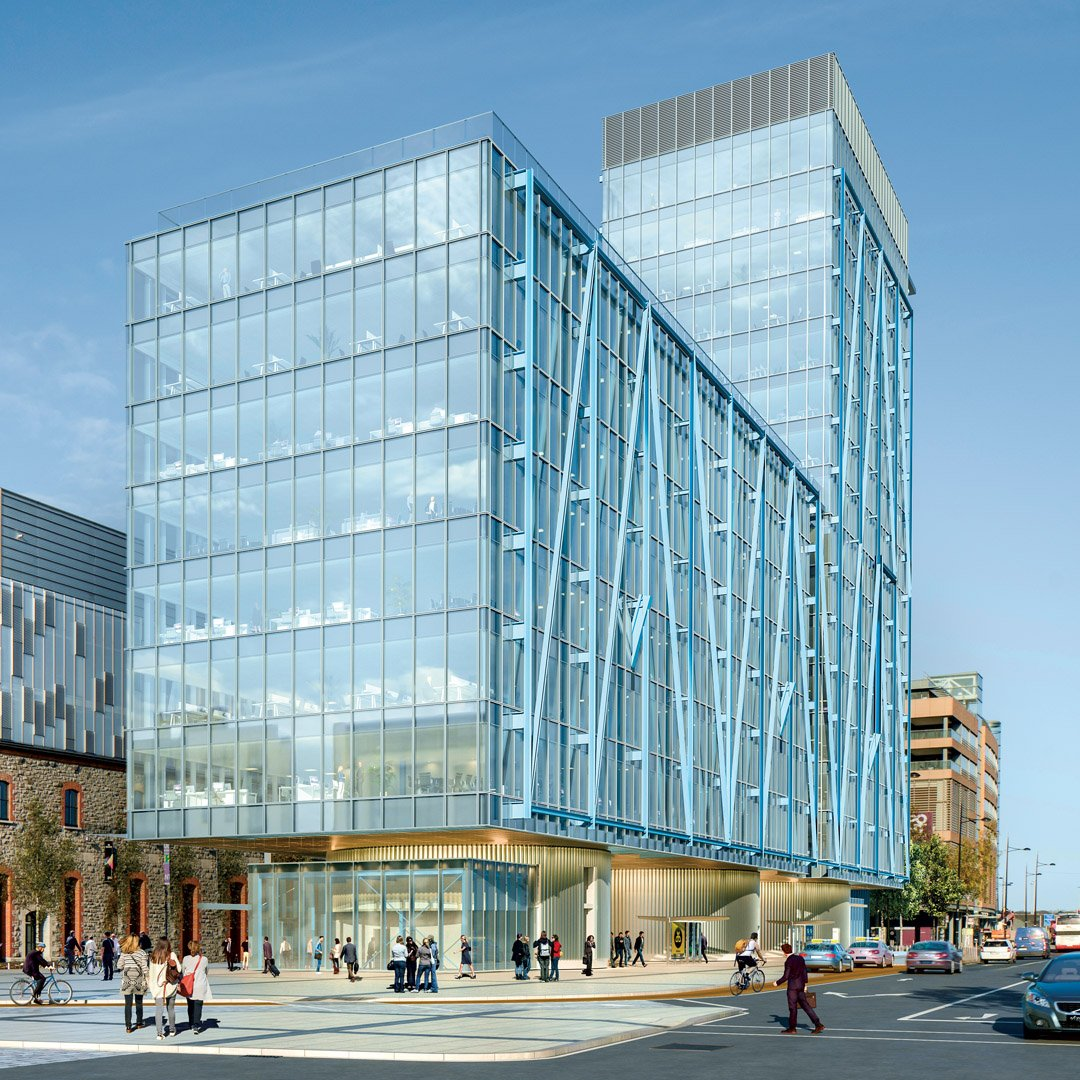
\includegraphics[width=\paperwidth,height=\paperheight]{exobuilding.jpg}}
\begin{frame}{Adaptable architecture and feedback loops}
%    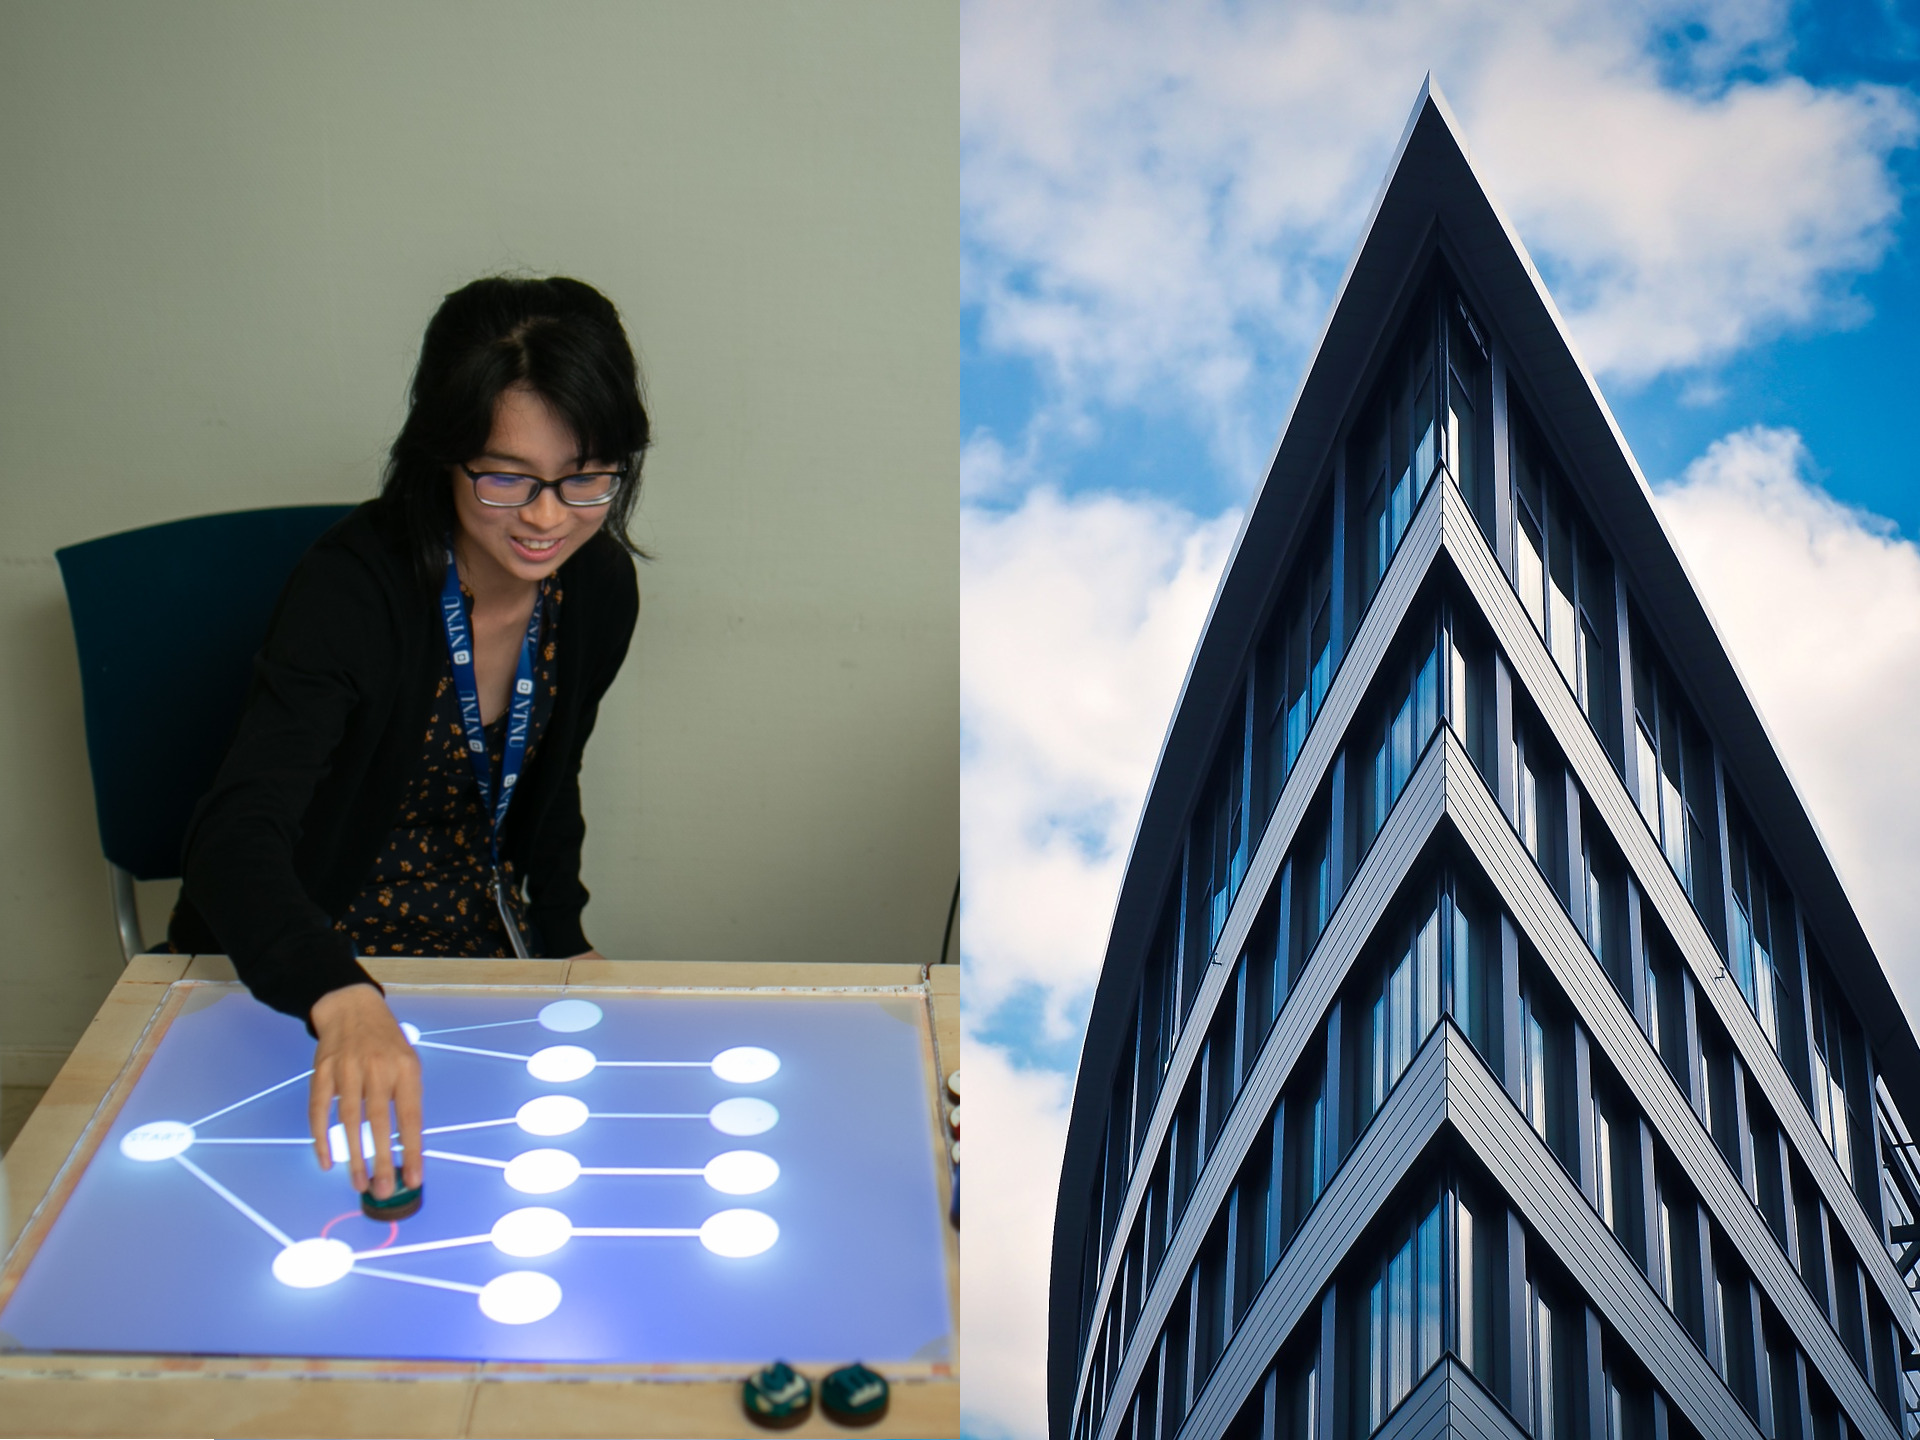
\includegraphics[width=\paperwidth,height=\paperheight]{interarch.jpg}%
%	\begin{block}{Intersection of architecture and interaction design}
    \source{\href{https://www.theexobuilding.com/}{The Exo Building Website}}
\end{frame}
}

%%%%%%%%%%%%%%%%%%%%%%%%%%%%%%%%%%%%%%%%%%%%%%%%%%%%%%%%%%%%%%%%%%%%%%%%%%%%%%%%%%%%%%%%%%%%%%%%

{
    \usebackgroundtemplate{\centering 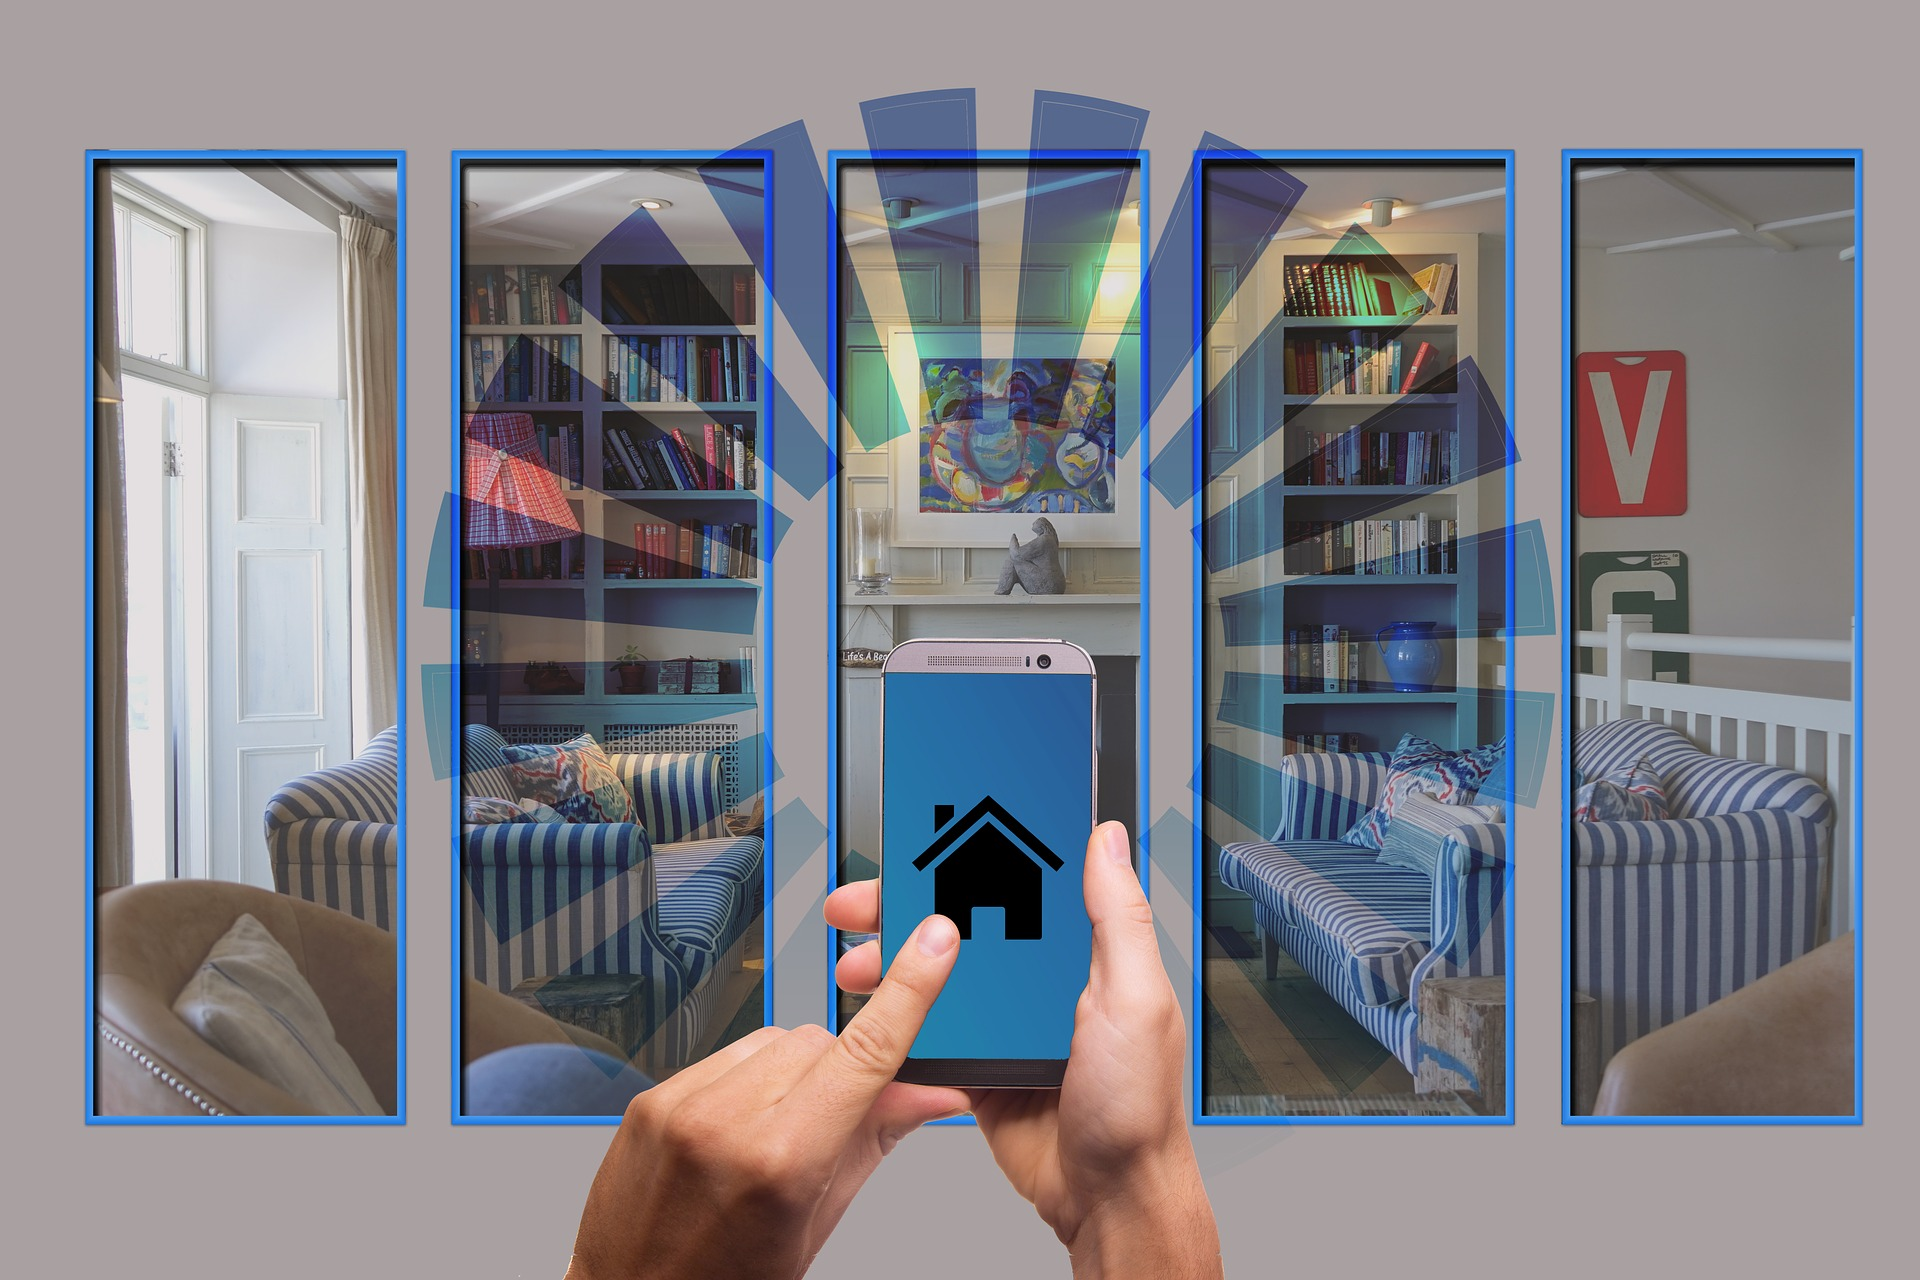
\includegraphics[width=\paperwidth,height=\paperheight]{smartbuilding.jpg}}
\begin{frame}{Improving communication between humans and buildings}
%    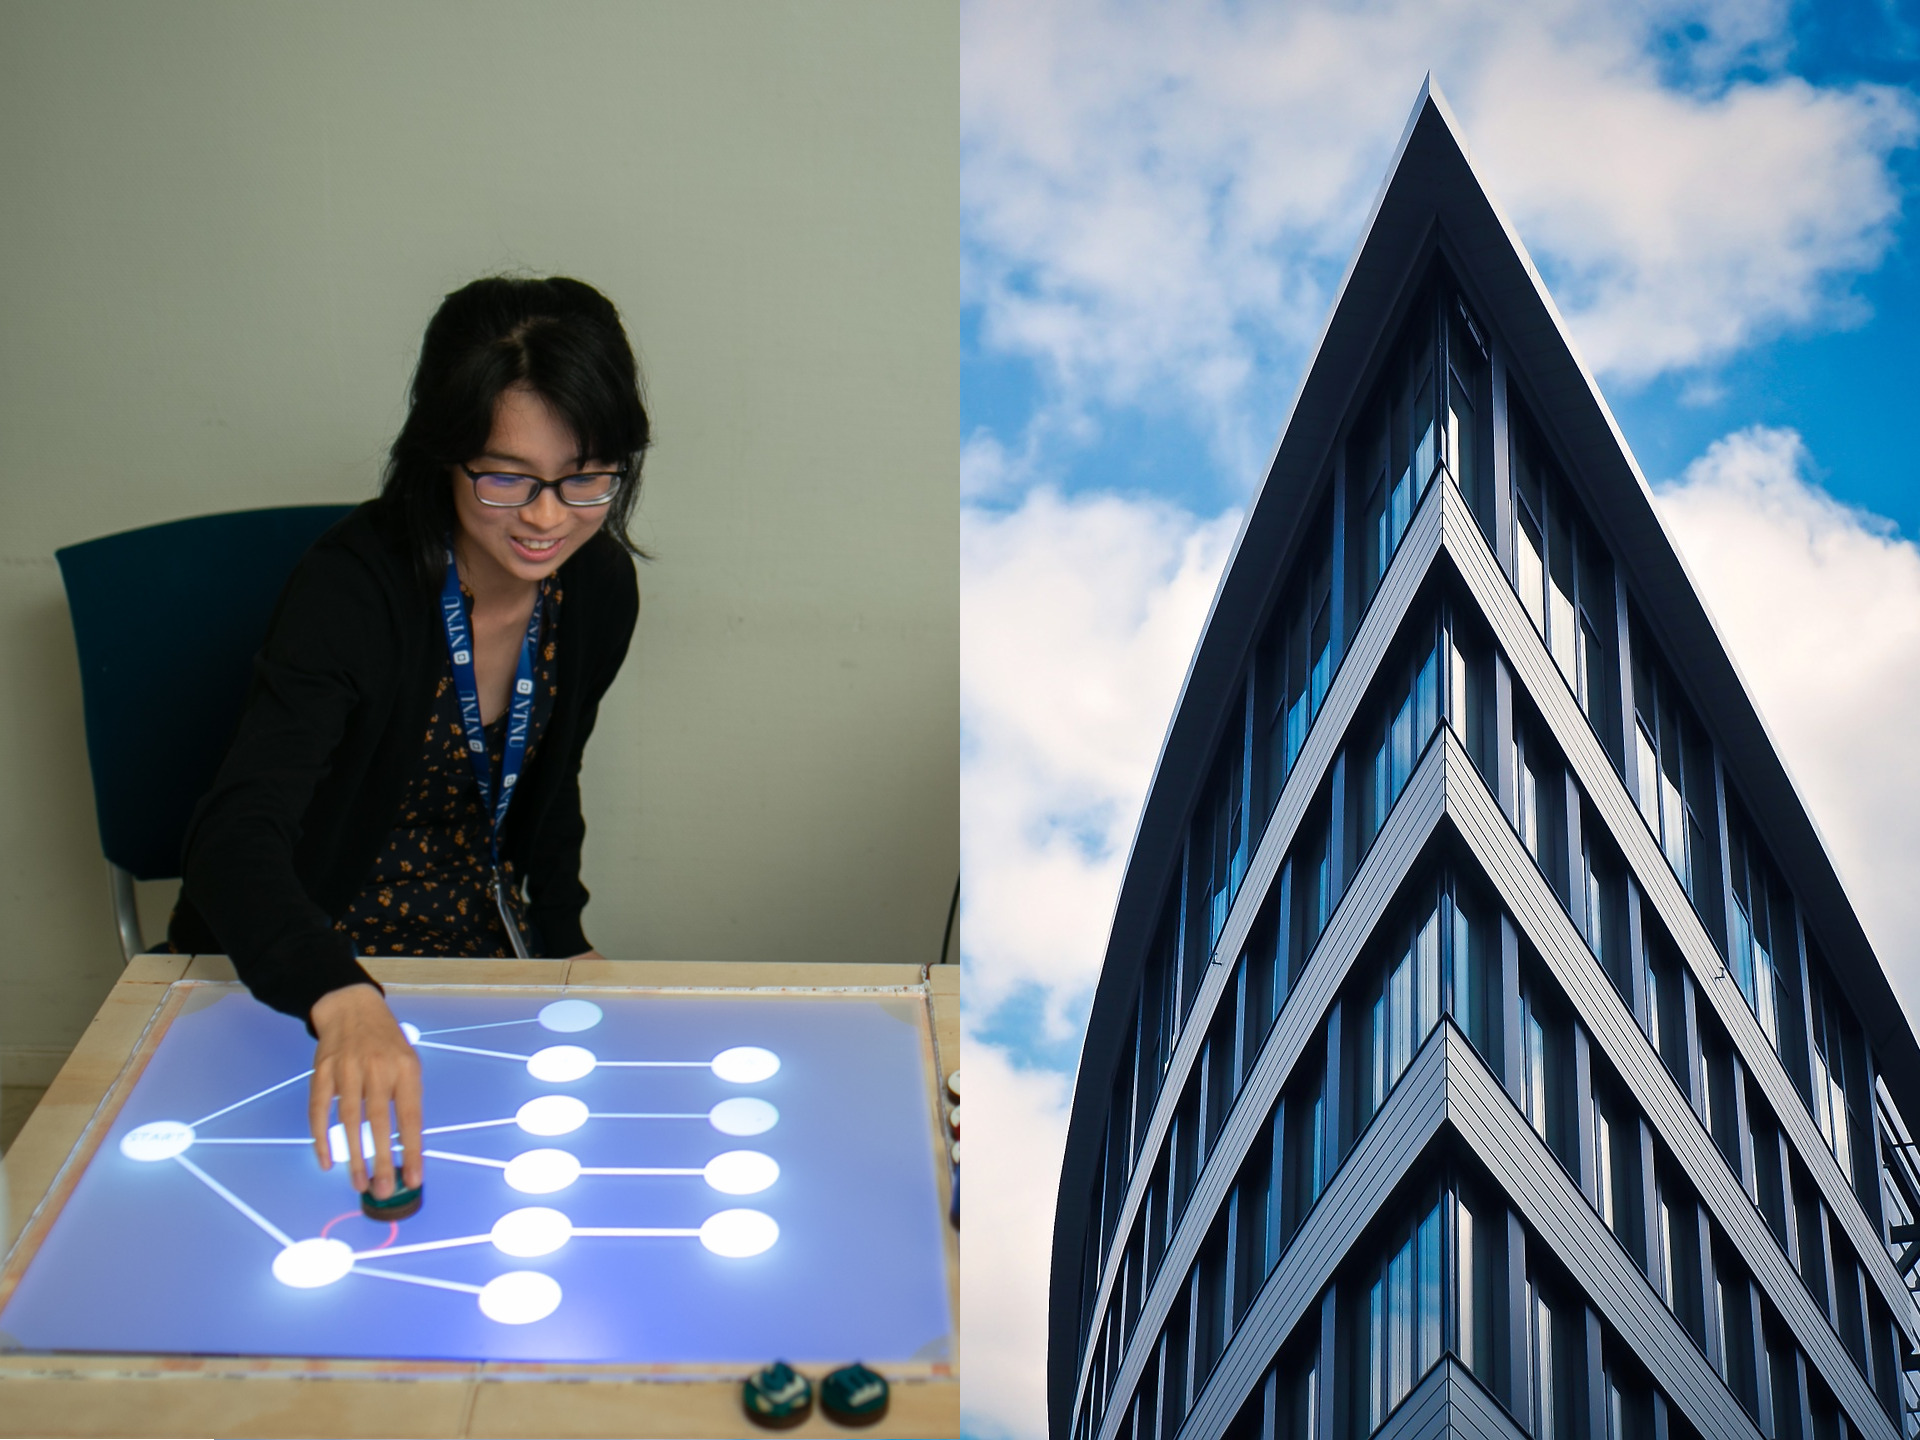
\includegraphics[width=\paperwidth,height=\paperheight]{interarch.jpg}%
%	\begin{block}{Intersection of architecture and interaction design}
    \source{\href{https://www.maxpixel.net/Technology-Multimedia-House-Smart-Home-Smartphone-3653454}{CC0 1.0 Max Pixel}}
\end{frame}
}

%%%%%%%%%%%%%%%%%%%%%%%%%%%%%%%%%%%%%%%%%%%%%%%%%%%%%%%%%%%%%%%%%%%%%%%%%%%%%%%%%%%%%%%%%%%%%%%%

\section{Short summary of SOTA}

%%%%%%%%%%%%%%%%%%%%%%%%%%%%%%%%%%%%%%%%%%%%%%%%%%%%%%%%%%%%%%%%%%%%%%%%%%%%%%%%%%%%%%%%%%%%%%%%

{
	\usebackgroundtemplate{\centering 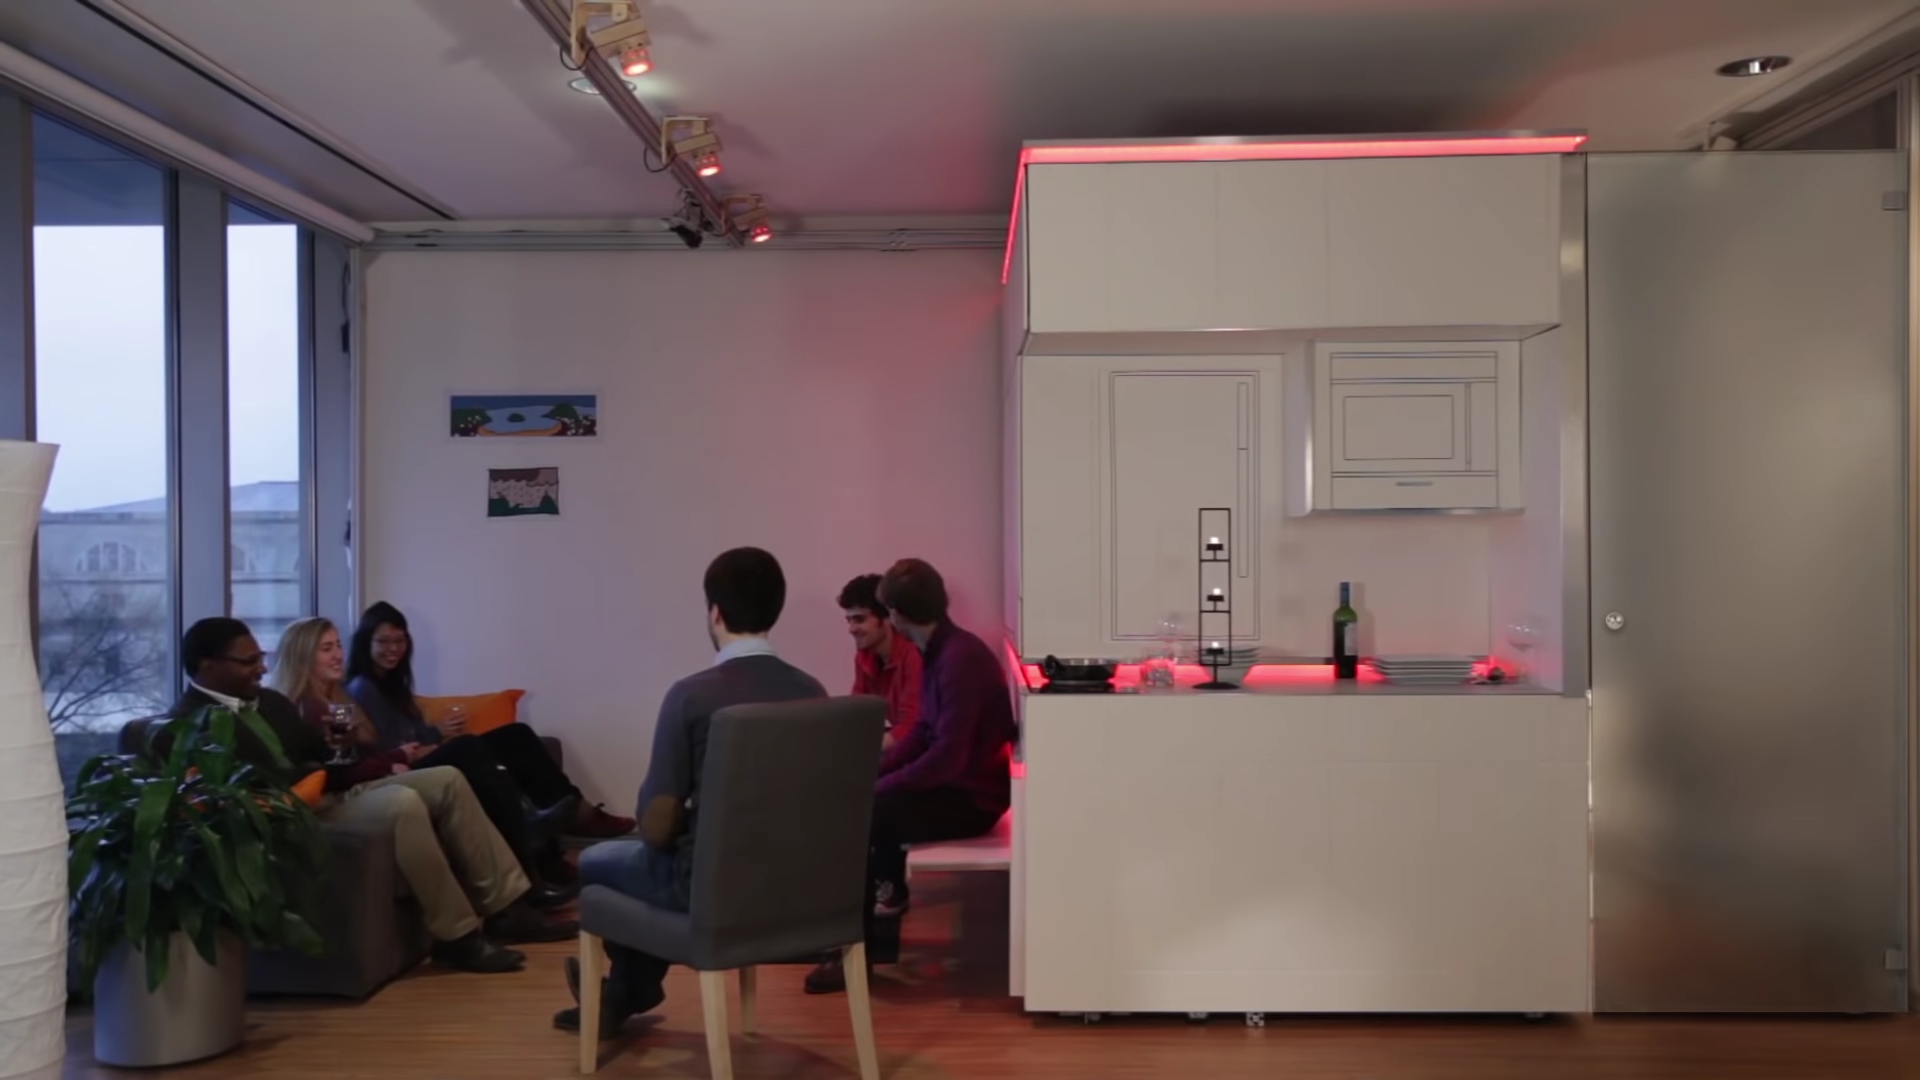
\includegraphics[width=\paperwidth,height=\paperheight]{images/cityhome/3.png}}
	\begin{frame}{Dynamic Livingspaces}
	
\end{frame}
}

%%%%%%%%%%%%%%%%%%%%%%%%%%%%%%%%%%%%%%%%%%%%%%%%%%%%%%%%%%%%%%%%%%%%%%%%%%%%%%%%%%%%%%%%%%%%%%%%

{
\usebackgroundtemplate{\centering 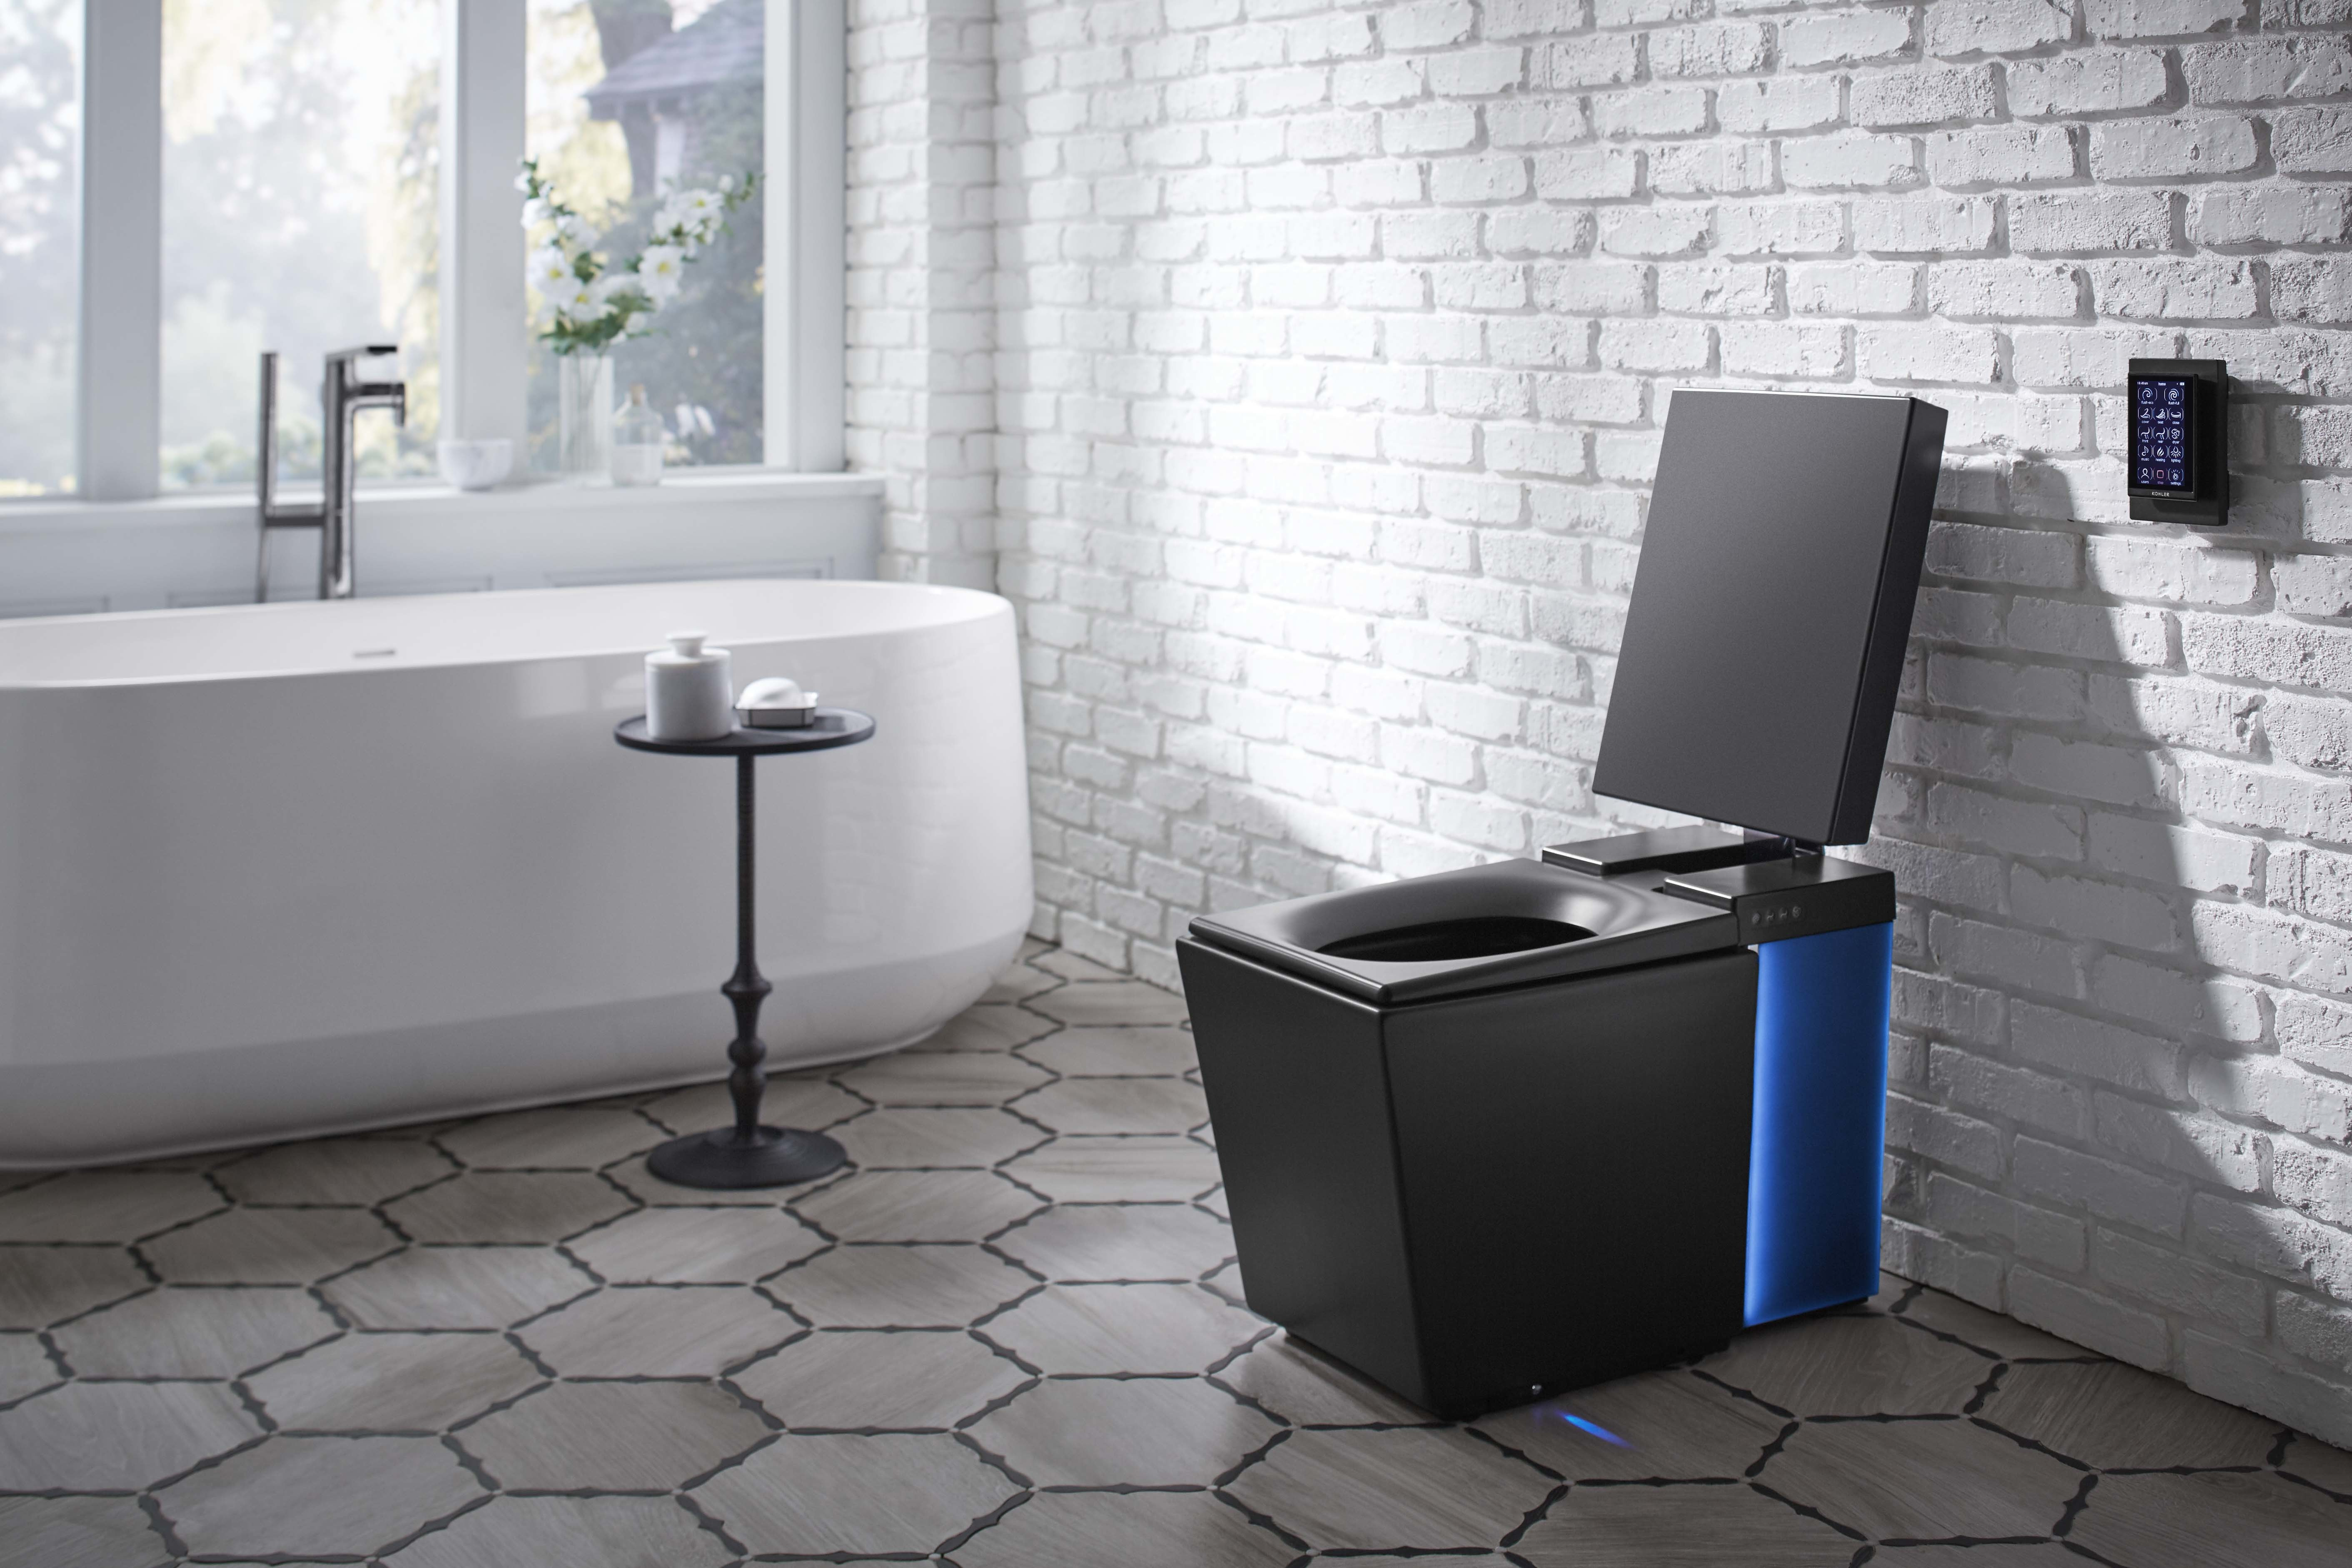
\includegraphics[width=\paperwidth,height=\paperheight]{images/numi/1.jpg}}
\begin{frame}{Improve Comfort and Health}

\end{frame}
}

%%%%%%%%%%%%%%%%%%%%%%%%%%%%%%%%%%%%%%%%%%%%%%%%%%%%%%%%%%%%%%%%%%%%%%%%%%%%%%%%%%%%%%%%%%%%%%%%

\begin{frame}{Implicit Interactions}
	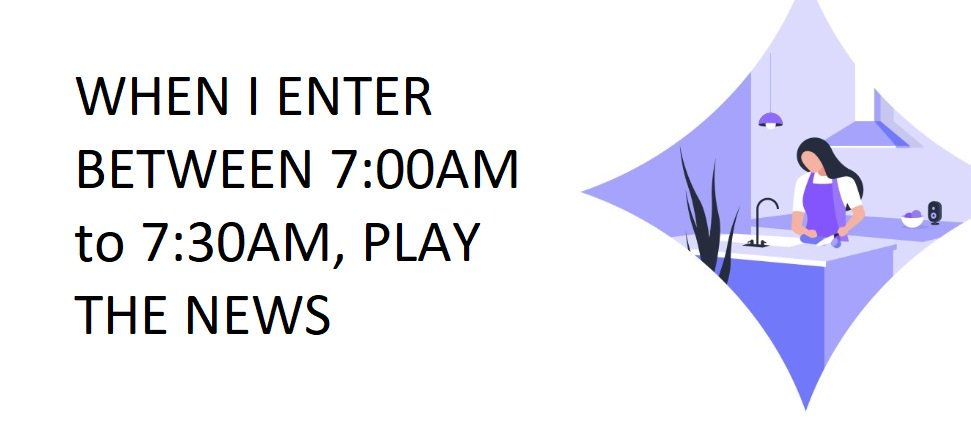
\includegraphics[width=\textwidth]{images/roomme/6.jpg}
\end{frame}

%%%%%%%%%%%%%%%%%%%%%%%%%%%%%%%%%%%%%%%%%%%%%%%%%%%%%%%%%%%%%%%%%%%%%%%%%%%%%%%%%%%%%%%%%%%%%%%%

{
	\usebackgroundtemplate{\centering 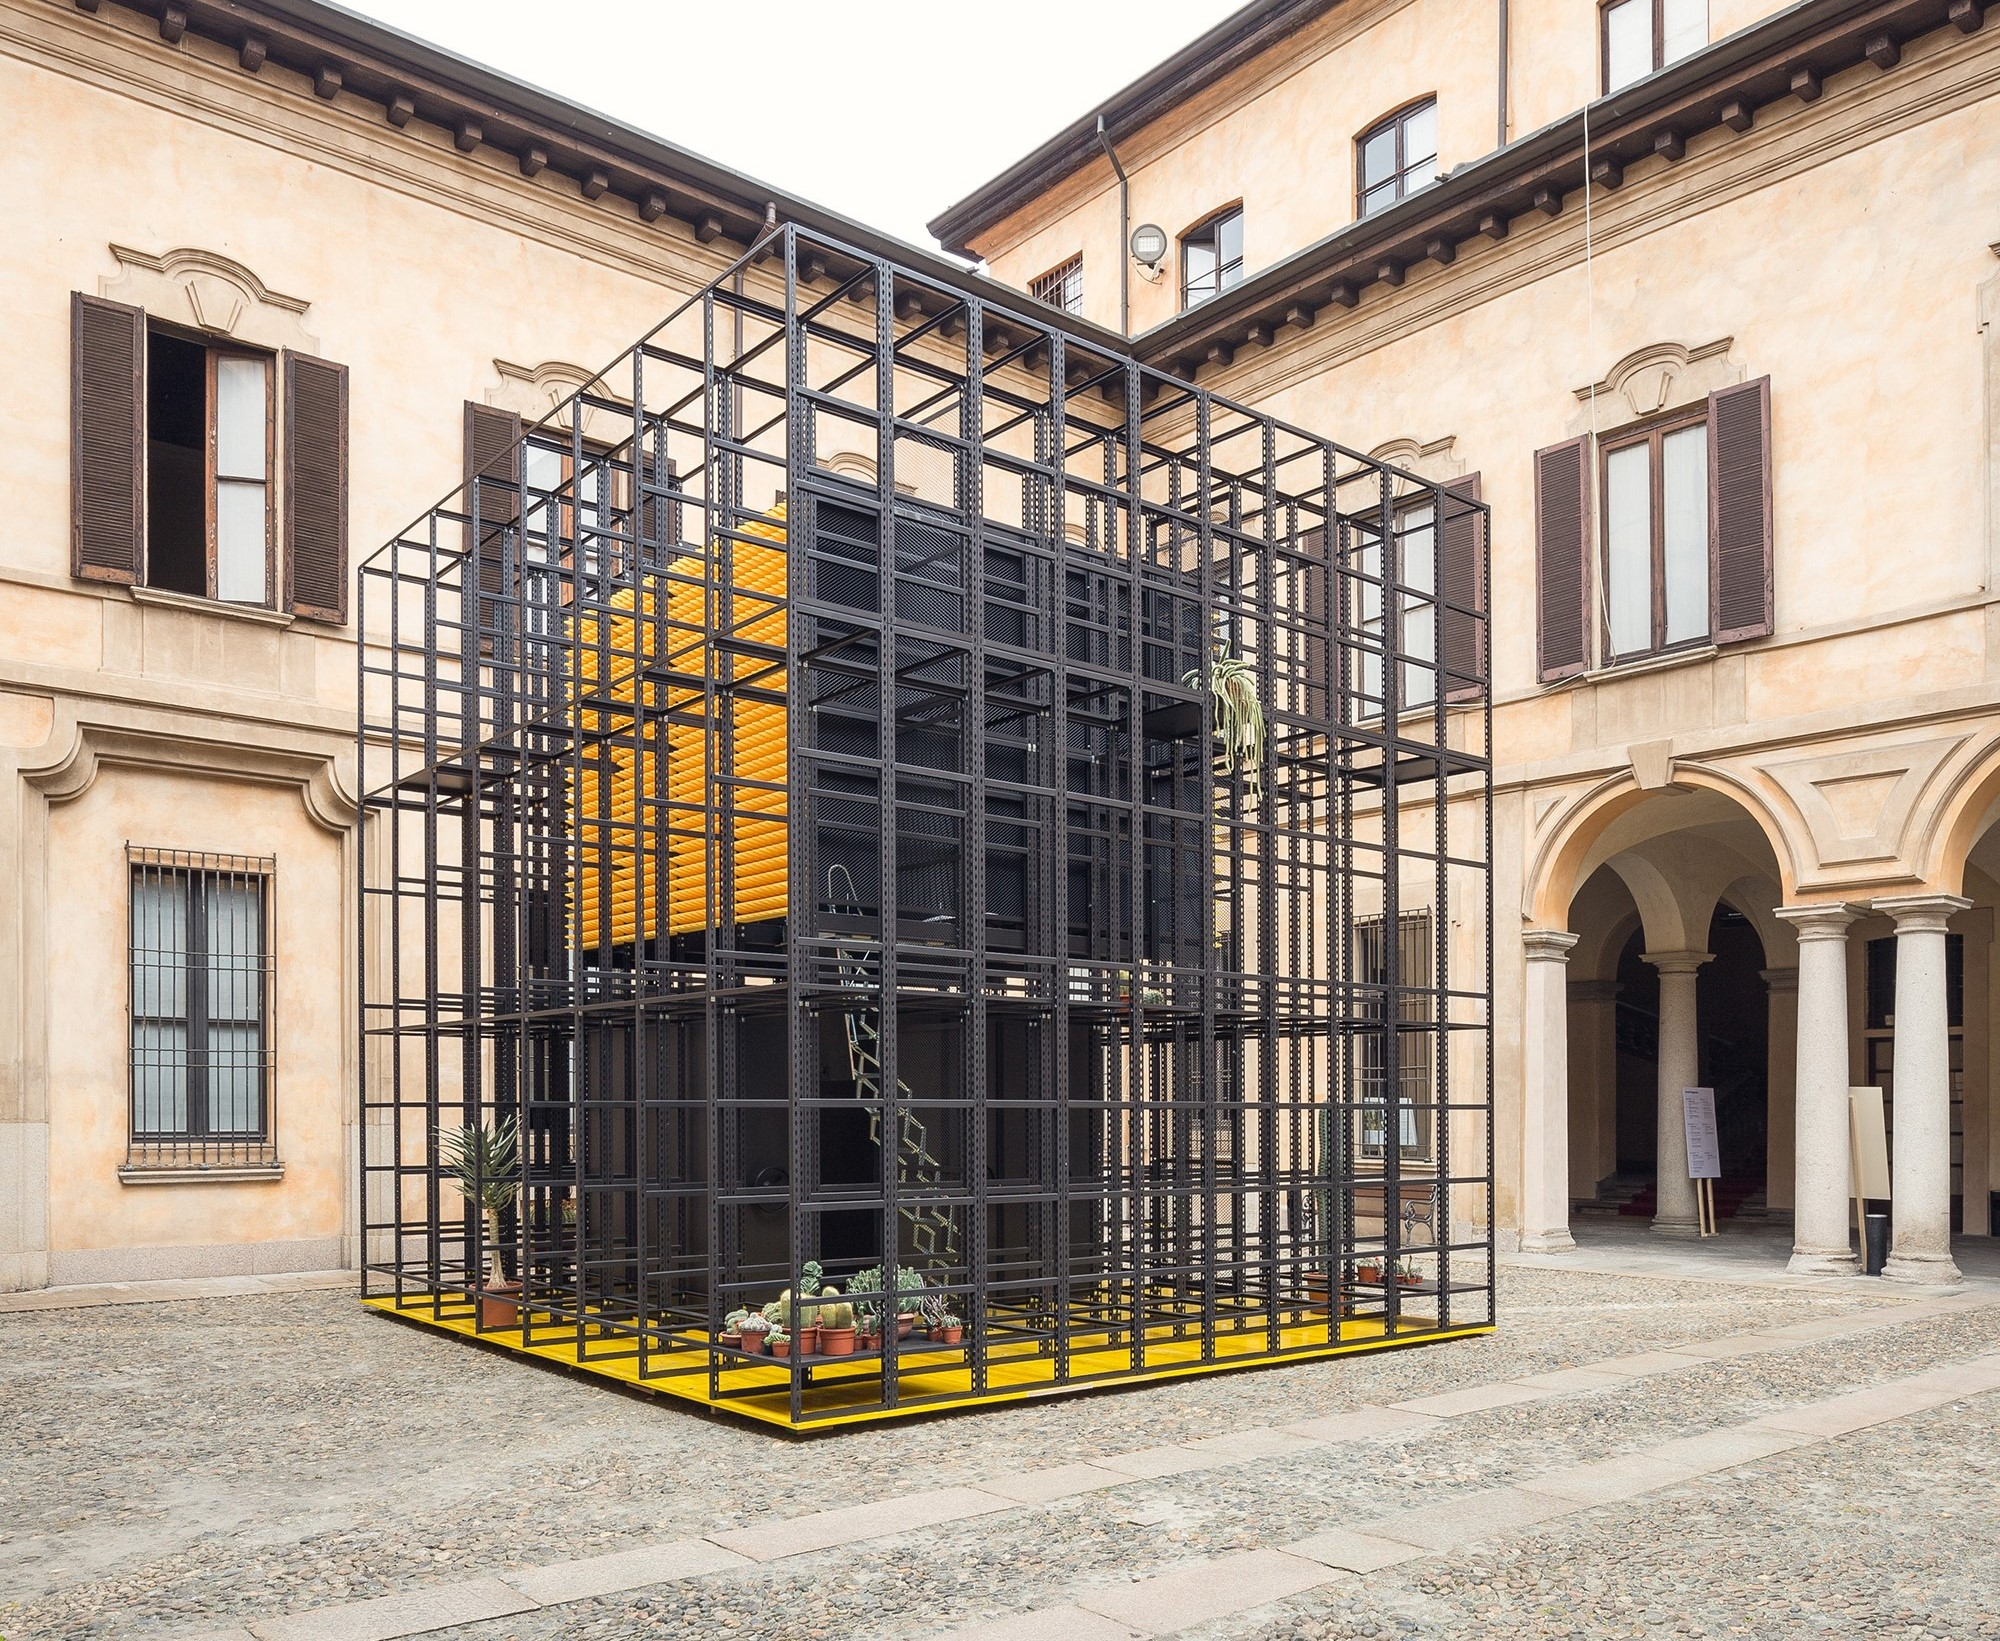
\includegraphics[width=\paperwidth]{images/ram-house/1.jpg}}
\begin{frame}{Privacy}
\end{frame}
}

%%%%%%%%%%%%%%%%%%%%%%%%%%%%%%%%%%%%%%%%%%%%%%%%%%%%%%%%%%%%%%%%%%%%%%%%%%%%%%%%%%%%%%%%%%%%%%%%

\begin{frame}{Privacy}
	\vspace{-4mm}
	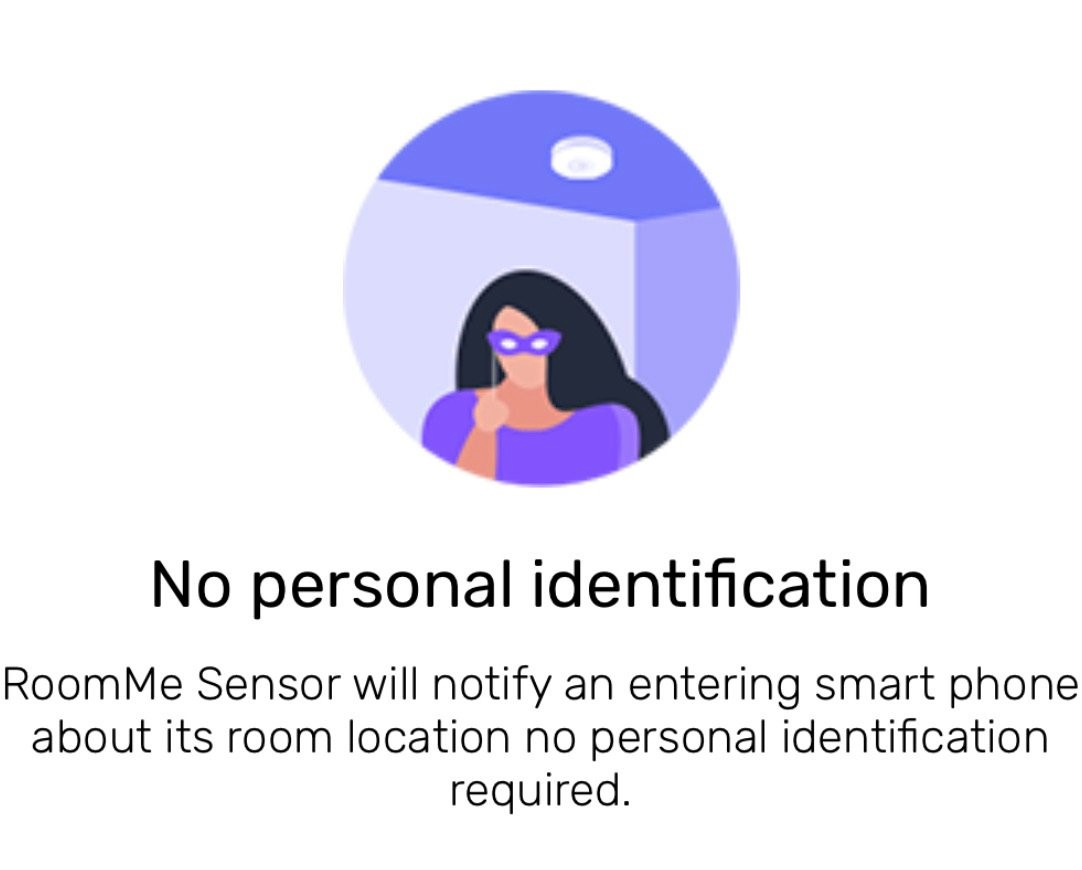
\includegraphics[width=\textwidth]{images/roomme/3.png}
\end{frame}

%%%%%%%%%%%%%%%%%%%%%%%%%%%%%%%%%%%%%%%%%%%%%%%%%%%%%%%%%%%%%%%%%%%%%%%%%%%%%%%%%%%%%%%%%%%%%%%%
\section{Introduction of expert and interview}
\begin{frame}{Holger Schnädelbach}
    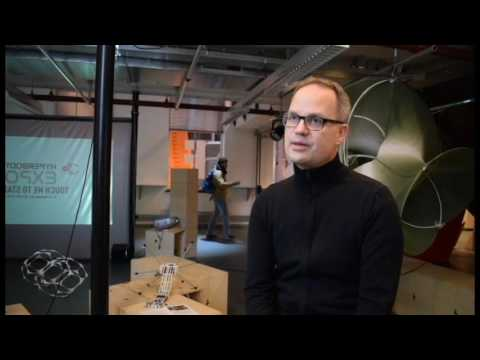
\includegraphics[width=\textwidth]{images/hoigi.jpg}
    \source{https://www.youtube.com/watch?v=p0BHUpTyDxU}
\end{frame}

%%%%%%%%%%%%%%%%%%%%%%%%%%%%%%%%%%%%%%%%%%%%%%%%%%%%%%%%%%%%%%%%%%%%%%%%%%%%%%%%%%%%%%%%%%%%%%%%



%%%%%%%%%%%%%%%%%%%%%%%%%%%%%%%%%%%%%%%%%%%%%%%%%%%%%%%%%%%%%%%%%%%%%%%%%%%%%%%%%%%%%%%%%%%%%%%%

\section{Findings of interview}
\begin{frame}{Findings}
    
\includegraphics[width=\textwidth]{images/interview.jpg}
    \source{http://picpedia.org/highway-signs/i/interview.html}
\end{frame}


%%%%%%%%%%%%%%%%%%%%%%%%%%%%%%%%%%%%%%%%%%%%%%%%%%%%%%%%%%%%%%%%%%%%%%%%%%%%%%%%%%%%%%%%%%%%%%%%



%%%%%%%%%%%%%%%%%%%%%%%%%%%%%%%%%%%%%%%%%%%%%%%%%%%%%%%%%%%%%%%%%%%%%%%%%%%%%%%%%%%%%%%%%%%%%%%%

\section{Personal reflections}

%%%%%%%%%%%%%%%%%%%%%%%%%%%%%%%%%%%%%%%%%%%%%%%%%%%%%%%%%%%%%%%%%%%%%%%%%%%%%%%%%%%%%%%%%%%%%%%%



%%%%%%%%%%%%%%%%%%%%%%%%%%%%%%%%%%%%%%%%%%%%%%%%%%%%%%%%%%%%%%%%%%%%%%%%%%%%%%%%%%%%%%%%%%%%%%%%
	%{\footnotesize \printbibliography}
  

%%%%%%%%%%%%%%%%%%%%%%%%%%%%%%%%%%%%%%%%%%%%%%%%%%%%%%%%%%%%%%%%%%%%%%%%%%%%%%%%%%%%%%%%%%%%%%%%

\end{document}
